
\mainsection{5}{Advanced optimization techniques}{15/05/2020}
\section{Difficulties in optimization }
\includegraphics[page = 134, width = \paperwidth]{PDFs/DL-Slides.pdf}
\includepdf[pages={135-142}, scale = 1,nup = 1x2 ]{PDFs/DL-Slides}
\includegraphics[page = 143, width = \paperwidth]{PDFs/DL-Slides.pdf}
2 Questions:
\textbullet universal approximation: Existence of a NN for each task\\
Will you find it?\\
\textbullet Why was the conventional NN not successful? \\
\putfigure{1.0}{1}{0.4}{Images/1DVisualizaitonOptimization}{1D Visualization Gradient Descent} 
%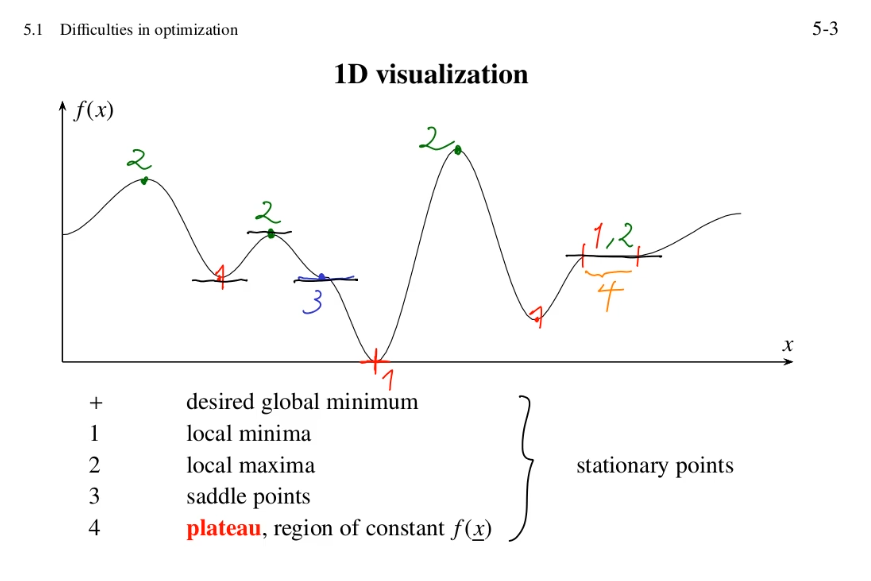
\includegraphics[width = \linewidth]{Images/1DVisualizaitonOptimization.png}\\
\putfigure{1.0}{1}{0.4}{Images/2DConturLines}{2D Contour lines} 
% 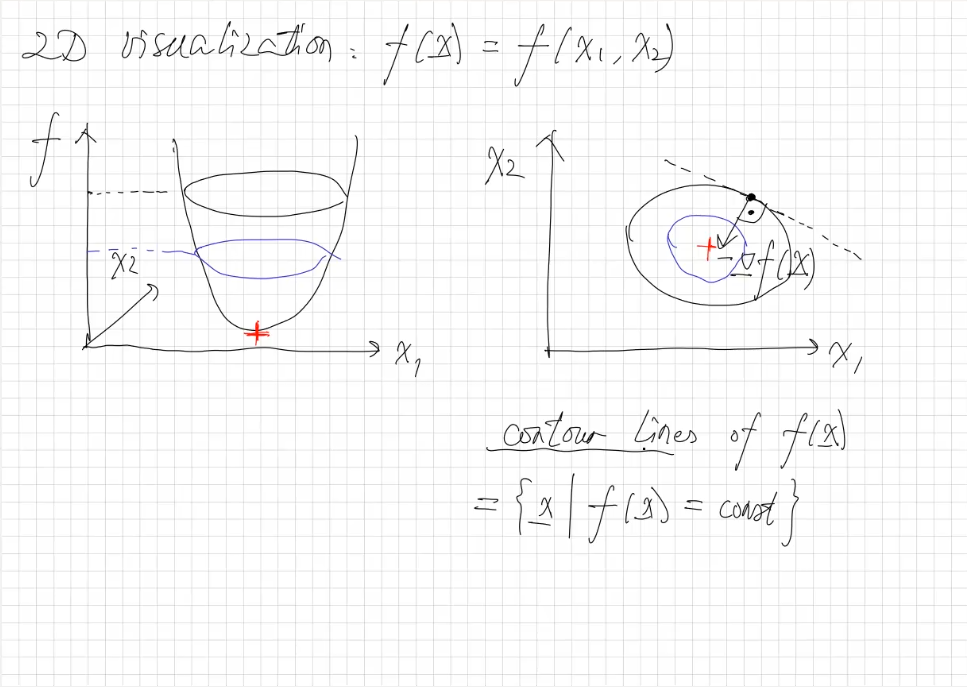
\includegraphics[width = \linewidth]{Images/2DConturLines.png}\\
\putfigure{1.0}{1}{0.4}{Images/IllConditioning}{Ill conditioning} 
%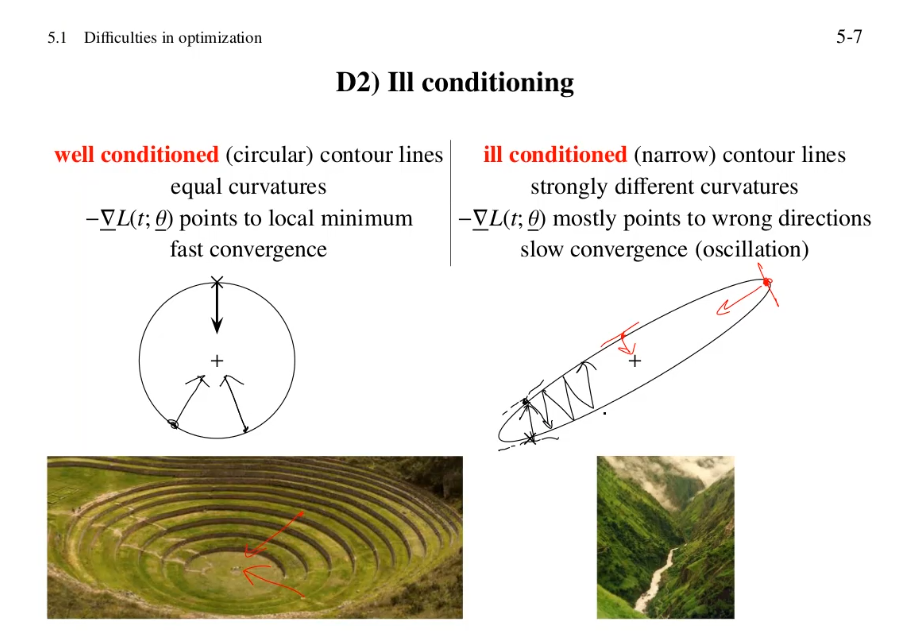
\includegraphics[width = \linewidth]{Images/IllConditioning.png}\\
\textbf{D3) Saddlepoint and plateau}
$  \underline{\nabla} L = \underline{0}  $ no update of $  \underline{x}^t $ because correction term is 0\\
in practice: $  \underline{\nabla} L \approx \underline{0} \rightarrow  $ very slow convergence\\
\putfigure{1.0}{1}{0.4}{Images/SensitiveChoiceStepsize}{Sensitive Choice for step size} 
%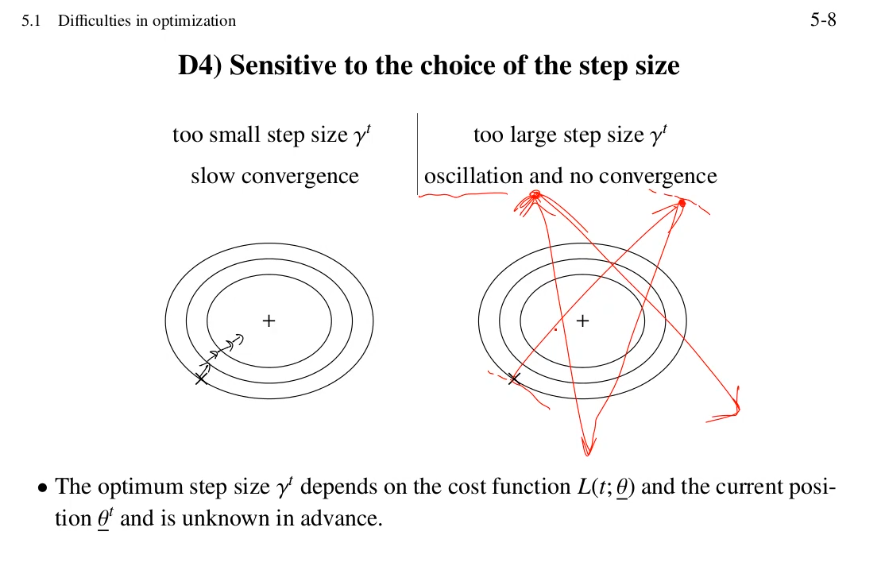
\includegraphics[width = \linewidth]{Images/SensitiveChoiceStepsize.png}\\
 \textbf{Vanishing Gradient:}\\
 Backpropagation of the error vector \\
 $  \Theta = \dfrac{\partial L (\underline{\theta}}{\partial \underline{a}_L} \in \Re^{1 \times M_L} $ in 4.7:\\
 $  \underline{\delta}_1^T = \underline{ \delta}_L ^T \cdot \underline{\underline{j}}_{\underline{a}_L} (\underline{a}_{L-1}),.., \underline{\underline{J}}_{\underline{a}_2} (\underline{a}_1) $, L Layers\\
 $ \underline{\underline{J}}_{\underline{a}_{L+1}} (\underline{a}_L) = \underline{\underline{J}}_{\underline{a}_{L+1}} (\underline{x}_l) \cdot \underline{\underline{J}}_{\underline{x}_L} (\underline{a}_L) = \underline{\underline{W}}_{l+1} \cdot diag( \phi'_{L} (\underline{a}_L))   $\\
 if $  || \underline{\underline{J}}_{\underline{a}_{L+1}} (\underline{a}_L) || < 1, \forall l $ matrix norm , then $  || \underline{\delta}_L || \rightarrow 0  $ \\
 vanishing gradient $\rightarrow$ no update of $  \underline{\theta}^T $ stop learning. 
 With the multiplication of a lot of terms smaller than 1 the gradient turns to a very small number close to zero \\
\textbullet if $  || \underline{\underline{J}}_{\underline{a}_{l+1}} (\underline{a}_l) || > 1, \forall l, $  then $ ||\underline{\delta}_l || \rightarrow \infty $\\
exploding gradient $\rightarrow$ divergence \\
no problem for shallow NN's because only small number of layers \\
bo problem for deep NN's because of large number of layers \\
\textbullet vanishing gradient less serious for the last layers $ (l \uparrow) $ \\
\textbullet more serious for first layers $ (l \downarrow) $ 
\subsection{E5.1: sigmoid vs. ReLU}
\textbf{a) sigmoid or tanh:} \\
$ \phi (a) = \sigma(a) = \dfrac{1}{1+ e^{-a}} \in (0,1) $ \\
if $ |a| >> 1: \phi'(a) \approx 0 $ due to saturation (shape of function )\\
$\rightarrow$ sigmoid bad for DNN die to vanishing gradient \\
\textbf{b) ReLU}\\
$  \phi (a) = max (0,a) $\\
$  \phi' (a) = \left\lbrace \begin{array}{lc}
1 & a > 0 \\
0 & a < 0
\end{array} \right. = u(a) $ \\
$\rightarrow$ ReLu less serious for vanishing gradient
\section{Momentum method}
\includegraphics[page = 144, width = \paperwidth]{PDFs/DL-Slides.pdf}
\includepdf[pages={145-146}, scale = 1,nup = 1x2 ]{PDFs/DL-Slides}
\includegraphics[page = 147, width = \paperwidth]{PDFs/DL-Slides.pdf}
an improvement of SGD \\
\textbullet change from $  \underline{\theta}^t $ to $ \underline{\theta} ^{t+1}: \Delta \underline{\theta}^t =\beta \cdot \Delta \underline{\theta}^{t-1}  \underbrace{  - \gamma^t \underline{\nabla}   L(t; \underline{\theta}) |_{\underline{\theta} = \underline{\theta}^t}}_{\text{gradient part}} $\\
\textbullet update: $  \underline{\theta}^{t+1} = \underline{\theta}^{t} + \delta \underline{\theta}^t $ \\
$  0 \leq \beta \leq 1 :  $ \textbf{momentum factor}\\
$  \beta =0 $ : SGD \\
$  \beta > 0  $ : recursive smoothing of $  \Delta \underline{\theta}^t $  \\
\textbf{Effect of the momentum: } \\
\textbullet reduce noise in stochastic gradient (D1) \\
\textbullet reduce oscillation and accelerate the convergence of the gradient method for ill conditioned contour lines(D2) 
\subsection{Nesterov Momentum}
a variant of momentum method \\
$  \Delta \underline{\theta} ^{t} =\beta \Delta \underline{\theta}^{t-1} +  \underbrace{(- \gamma^t \underline{ \nabla} L(t; \underline{\theta})|_{ \underline{\theta} = \underline{\theta}^t + \beta \Delta \underline{\theta}^t)}}_{\text{lookahead gradient at the predicted position } \underline{\theta}^{t-1} + \beta \Delta \underline{\theta}} $ 
\section{Learning rate schedule}
\includegraphics[page = 148, scale=.6]{PDFs/DL-Slides.pdf}\\
\includegraphics[page = 149, scale=.6]{PDFs/DL-Slides.pdf}\\
How to choose the step size /learning rate $  \gamma^t $?\\
Many possible schedules \\
\textbf{S1 constant learning rate:}\\
$ \gamma^t = \gamma = const., \forall t $\\
But difficulty D4: \\
\textbullet $  \gamma $ too small: slow convergence \\
\textbullet $  \gamma $ too large: no convergence / oscillation around local minimum\\
$\rightarrow$ Need a trade-off between \\
\textbullet fast convergence at the beginning: $  \gamma \uparrow $ (large step size) \\
\textbullet less oscillation afterwards : $  \gamma \downarrow $ reduce stepsize with growing number of iterations: \textbf{learning rate decay} \\
\textbf{Weakness:}\\
\textbullet manual choice of $ \gamma_0, t_0 , c $\\
\textbullet same schedule for all parameters in $ \underline{\theta} $ \\
\textbf{Adaptive schedules:}
\textbullet different schedules for different parameters in $  \underline{\theta} $\\
\textbullet $ \gamma^t  $ calculated dynamically depending on $ \underline{\theta}^t $ \\
Slide 5-16 Adam very popular 
\section{Input and batch normalization}
\includegraphics[page = 150, width = \paperwidth]{PDFs/DL-Slides.pdf}
\includepdf[pages={151-154}, scale = 1,nup = 1x2 ]{PDFs/DL-Slides}
\subsection{E5.3 A Perceptron}
a) large offset : $  \x (n) = \underset{offset}{\x_0} + \tilde{\x} (n) , || \x _ 0 || >> \tilde{\x} (n) , \forall n  $\\
$\rightarrow \underline{\underline{R}} \approx \x_0 \x_0^T ,$ rank one \\
b) strongly different variances: e.g $  \x(n) = \left[ \begin{matrix}
large \\
small \\
\vdots \\
small
\end{matrix} \right]  \sim \left[ \begin{matrix}
1 \\
0 \\
\vdots \\
0 
\end{matrix} \right] = \e_1 , \forall n$ \\
$\rightarrow \underline{\underline{R}} \sim \e, \e^T , $ rank one \\
\textbf{AM:} $ \RR  $ has approximately rank one \\
$\rightarrow  \RR $ has one large eigenvalue $  \lam_1 $ with eigenvector $  \v_1 = \x_0 $ or $ \v_1 \sim \e_1 $ and d-1 small eigenvalues\\
$\rightarrow $ very narrow contour lines \\
$ \rightarrow $ slow convergence (D2)\\
\textbf{Need input normalization}, e.g.: zero-mean unit-variance normalization \\
For each $  x_i(n)  = [ \x_0 (n)] _i, 1 \leq n \leq N$\\
$  x_i(n) \leftarrow \dfrac{x_i (n)- \mu_i}{\sigma_i} $ with estimated mean $  \mu_i = \dfrac{1}{N} \sum_{n=1}^{N} x_i (n) $ \\
variance $  \sigma_i^2 = \dfrac{1}{N-1} \sum_{n=1}^{N} (x_i (n) - \mu_i )^2 $ (N-1 because unbiased mean wanted)
\textbullet normalization for the whole training set D \\
\textbullet equally for all channels $ x_i $\\
Advantage: \\
\textbullet no ill conditioning (D2) \\
\textbullet faster convergence 
\subsection{Batch normalization}
Input normalization: done once for the data set \\
Hidden layers: data distribution changes\\
\textbullet over layers  \\
\textbullet over time during training 
those to points are called internal covariate shift \\
$ \rightarrow $ slower convergence  \\
\textbf{Batch normalization(BN):} : like input normalization \\
\textbullet for any hidden layer \\
\textbullet for each mini batch of length B \\
\putfigure{1.0}{1}{0.2}{Images/SketchMiniBatchNormalization}{Sketch for mini batch normalization } \\
\putfigure{1.0}{1}{0.45}{Images/SummaryBatchNormalization}{Summary BN} \\
\putfigure{1.0}{1}{0.45}{Images/SummaryBatchNormalization2.png}{Summary BN 2} 
\section{Parameter initialization}	
\includegraphics[page = 155, width = \paperwidth]{PDFs/DL-Slides.pdf}
SGD does a local search: The solution depends on the initial value $  \theta ^0 $ \\
$  \Theta ^0 = ?? $
\textbf{2 Random onotialization of $ \W_L $} , e.g.
\textbullet normal or Gaussian distribution $ N() $\\
$ [ \W_L ]_{ij} \sim $ i.i.d (independent identically distributed) $  \sigma \cdot N(0,1) = N (0, \sigma^2)$\\
\textbullet uniform distribution $  U(\cdot) $ \\
$  [\W_L]_{ij} \sim  $ i.i.dl $  \sigma U(-1,1 ) = U(\sigma, \sigma) , \sigma = const, \forall l,i,j $ \\
$ \rightarrow $ not optimal \\
3) He initialization \\
as 2) , but $ \delta_l \sim \dfrac{1}{\sqrt{M_{L-1}}} $  $ \rightarrow $ constant activation flow after initialization \\
layer $  l $ : $ \a_l = \W_l \cdot \x _{l-1} + \b_{l} \overset {\b = \underline{0}}{=} \W_l \cdot \x_{l-1} $ or \\
$  \a = \W \cdot \x , \\
\a = [a_i] \in \R ^{M_l} $\\
$  \W = [w_{ij}] \in \R^{M_l \times M_{l-1}} $\\
$  \x = [x_i ] \in \R^{M_{l-1}} $\\
	$ \rightarrow  a_i = \sum_{j=1}^{M_{l-1}} w_{ij} \cdot x_j$\\
Assumptions:\\
\textbullet $ x_i  $ i.i.d zero mean , variance $  \sigma_x^2 $ \\
\textbullet $  w_{ij}  $  i.i.d zero mean , variance $  \sigma_w^2 $ \\
\textbullet $  x_i  $ and $  w_{ij} $ independent \\
$ \rightarrow $ \textbullet $  E(a_i) = \sum_{j}^{} E(w_{ij}) \cdot E(x _{ij} ) = 0$\\
\textbullet $  Var(a_i)  = E(a_i^2) = E (\sum_j w_{ij} \cdot x_j )^2 = E(\sum_j \sum_k w_{ij} w_{ik} x_{j} x_{k} ) = \sum_j \sum_k E(w_{ij} w_{ik} \cdot E(x_j x_k))  = \sum_{j=1}^{M_{l-1}} \sigma_w^2 \cdot \sigma_x^2 = M_{l-1} \cdot  \sigma_w^2 \cdot \sigma_x^2 $\\
\textbf{constant activation flow } $  \equiv  $ smooth information flow in the forward pass \\
$ Var (a_i) = const. , \forall i,l  $\\
$ \rightarrow \sigma_{w,l} \sim \dfrac{1}{\sqrt{M_{l-1}}}$, $ M_{l-1}:  $ fan-in\\
\textbf{4) Glorot initialization }\\
const. gradient flow in backward pass \\
$ ||  \dfrac{\partial L }{\partial \a_l}|| = const, \forall l$ $ \rightarrow  \sigma_{w,l} \sim \dfrac{1}{\sqrt{M_l}}, M_l:$ fan-out\\
compromise: $  \sigma_{w,l} \sim \dfrac{1}{\sqrt{M_{l-1} + M_l}} $
\section{Improved (network)-model}
\includegraphics[page = 156, width = \paperwidth]{PDFs/DL-Slides.pdf}
\includepdf[pages={157-160}, scale = 1,nup = 1x2 ]{PDFs/DL-Slides}
A) Better activation functions $  \phi(\cdot) $, e.g. \\
\textbullet ReLU instead of sigmoid \\
\textbullet leaky reLu instead of ReLU\\
\textbf{B) skip connections, shortcuts , residual network (ResNet)}\\
\putfigure{1.0}{1}{0.45}{Images/LayerSkip}{Layerskip / shortcuts } \\
\textbullet backward pass<. no vanishing gradient over identity path. \\
$  \x_l = \phi_l (\W \x_{l-1} + \b_l )  + \x_{l-1}$\\
$ \dfrac{\partial \x_l}{\partial \x_{l-1} = \dfrac{\partial \phi _l (\cdots)}{\partial \x_{l-1}}} + \II  $\\
c) Many other architecture improvements see ch.10 




 

























